\documentclass{beamer}

\usepackage{amsmath}
\usepackage{amssymb}
\usepackage{mathtools}
%\usepackage{float}
\usepackage[pdftex]{graphicx}
%\usepackage{ngerman}
\usepackage[T1]{fontenc}
\usepackage[utf8]{inputenc}
\usepackage{enumerate}
\usepackage{ifpdf}

\usetheme{Warsaw}

\title{Elektronikpraktikum Auswertung: Versuch 2}
\author{Gruppe 1 \\ Patrick Heuer \\ Benjamin Lotter}
\date{}

\begin{document}
\maketitle
%\tableofcontents

\begin{frame}
\frametitle{Aufgabe 1}
\framesubtitle{Bestimmung von komplexem Widerstand und Phase}
    \begin{itemize}
        \item Bestimmung des Widerstands durch Messung von Strom und Spannung
        \item Strommessung = Spannungsmessung an bekanntem Widerstand
    \end{itemize}    
    \begin{figure}[H]
    \begin{center}
            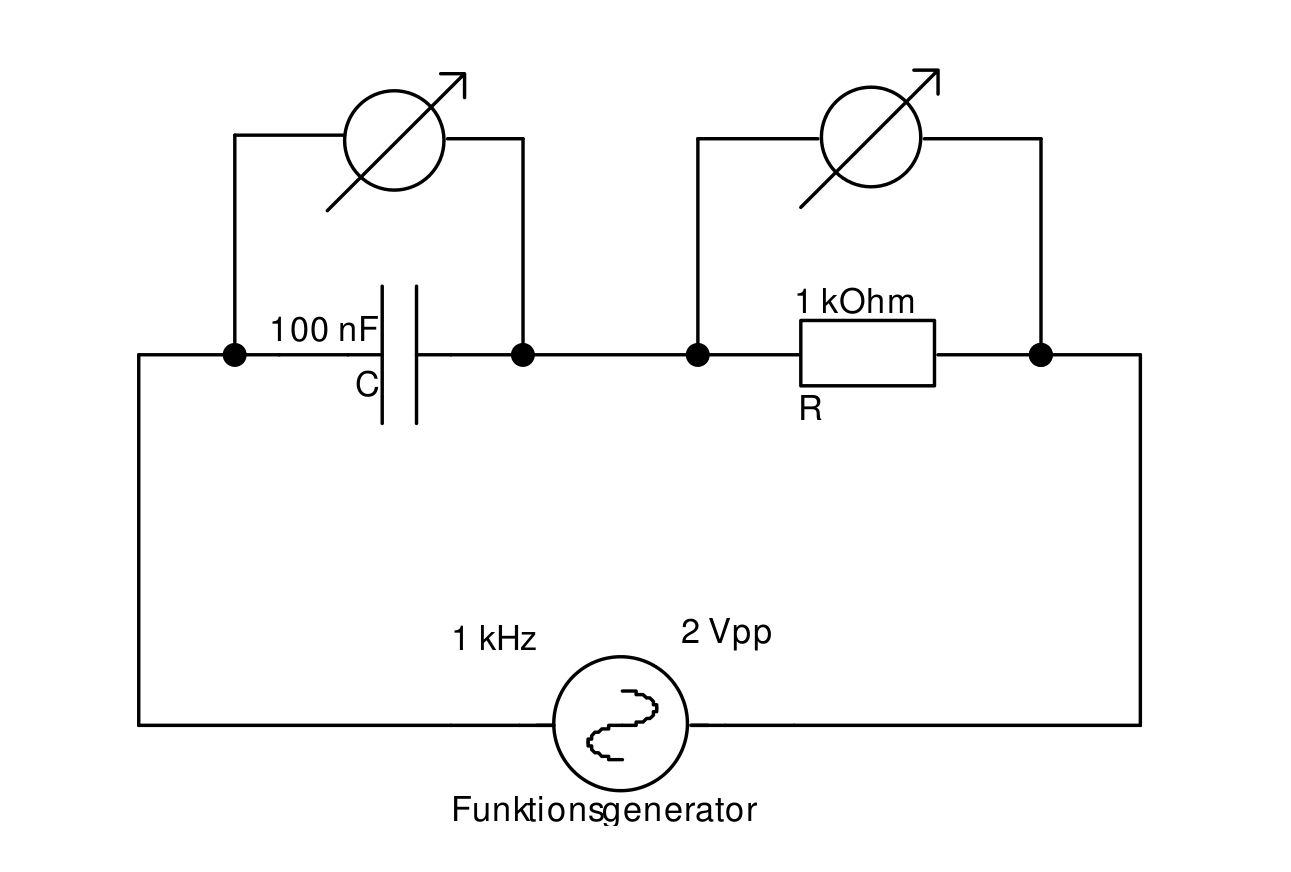
\includegraphics[scale=0.15]{./img/schaltbild_1_ohne_erdung.png}
    \end{center}
    \end{figure}
\end{frame}
\begin{frame}
\frametitle{Aufgabe 1}
\framesubtitle{Bestimmung von komplexem Widerstand und Phase}
    \begin{itemize}
        \item Problem: Erdschleife
    \end{itemize}
    \begin{figure}[H]
    \begin{center}
            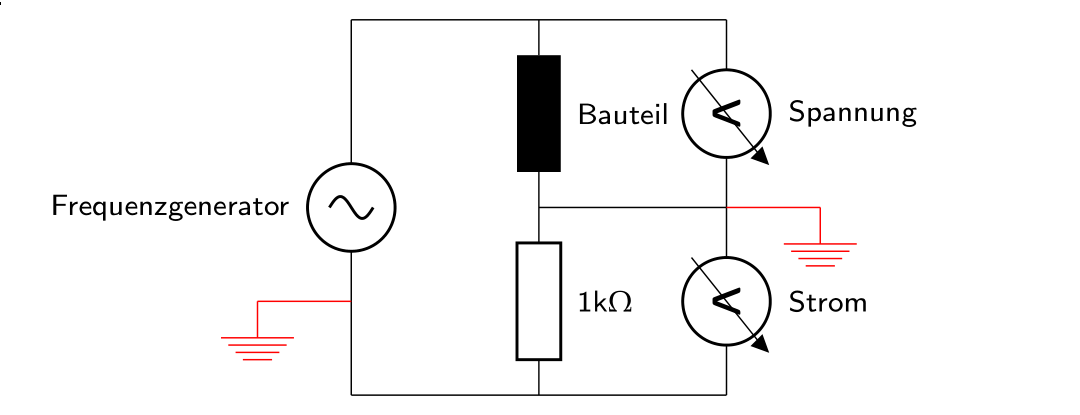
\includegraphics[scale=0.3]{./img/schaltbild_1_alle_erdungen.png}
    \end{center}
    \end{figure}
\end{frame}
\begin{frame}
\frametitle{Aufgabe 1}
\framesubtitle{Bestimmung von komplexem Widerstand und Phase}
    \begin{itemize}
        \item Problem: Erdschleife
        \item Lösung: Erdungen aufeinander legen
        \item Abfall über Bauteil: "Math function 2 - 1"
    \end{itemize}
    \begin{figure}[H]
    \begin{center}
            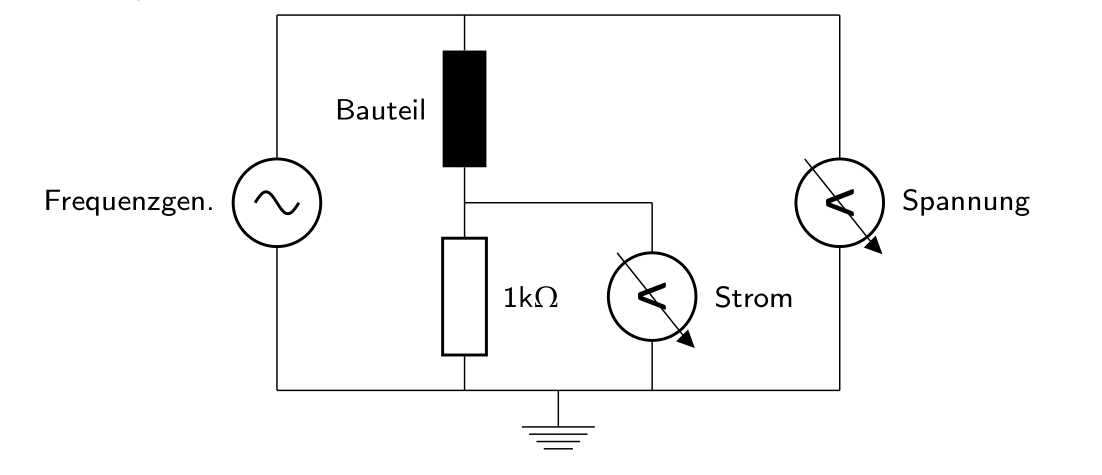
\includegraphics[scale=0.3]{./img/schaltbild_1_mit_erdschleife.png}
    \end{center}
    \end{figure}
\end{frame}

\begin{frame}
\frametitle{Aufgabe 1}
\framesubtitle{Kondensator}
\begin{figure}[H]
    \begin{center}
                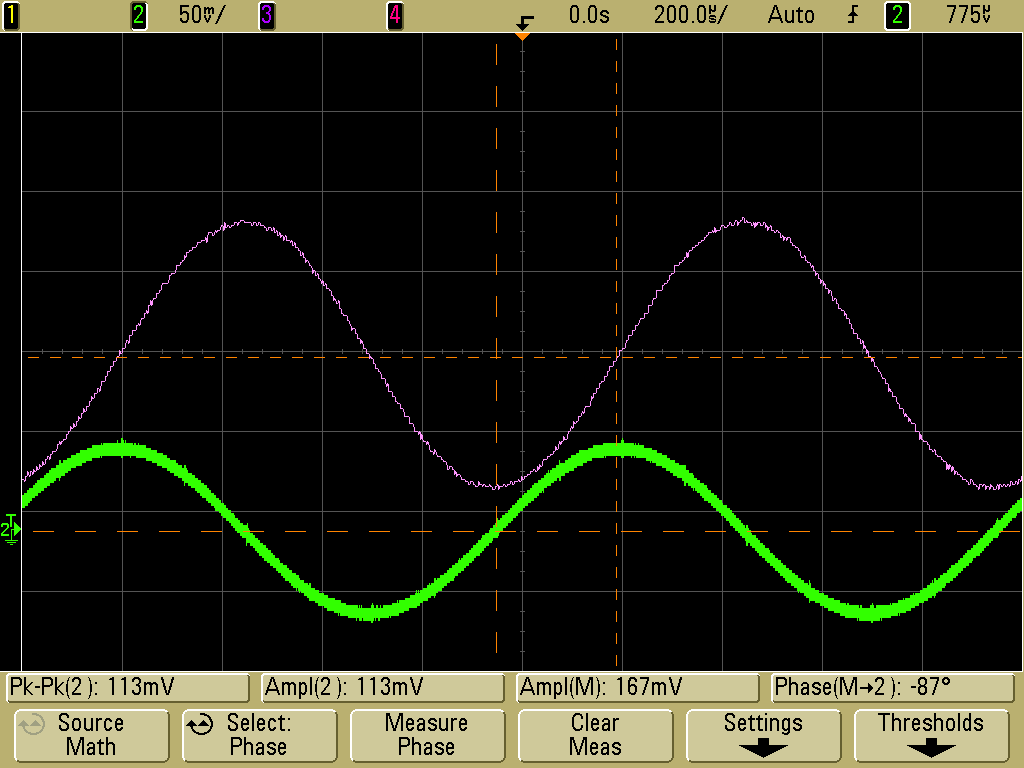
\includegraphics[scale=0.15]{./img/1a_Kondensator_1.png}
    \end{center}
\end{figure}
\begin{center}
\begin{tabular}{c|| c | c | c}
    & $I$ & $U$ & $\varphi$ \\
    \hline
    Kondensator ($100nF$)& $113 \mu A$ & $167mV$ & $-87^{\circ}$ \\
\end{tabular}
\end{center}
\end{frame}

\begin{frame}
\frametitle{Aufgabe 1}
\framesubtitle{Spule}
\begin{figure}[H]
    \begin{center}
                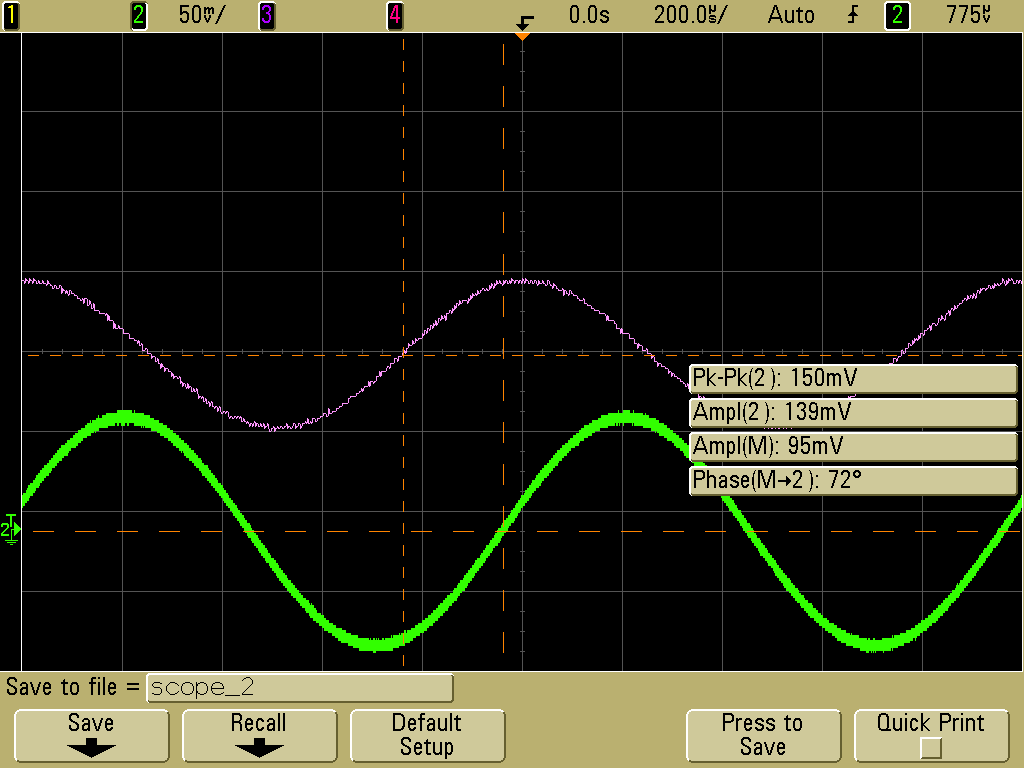
\includegraphics[scale=0.15]{./img/1b_Spule.png}
    \end{center}
\end{figure}
\begin{center}
\begin{tabular}{c|| c | c | c}
    & $I$ & $U$ & $\varphi$ \\
    \hline
    Kondensator ($100nF$)& $113 \mu A$ & $167mV$ & $-87^{\circ}$ \\
    Spule ($100mH$)& $139 \mu A$ & $95 mV$ & $72^{\circ}$ 
\end{tabular}
\end{center}
\end{frame}

\begin{frame}
\frametitle{Aufgabe 1}
\framesubtitle{Widerstand}
\begin{figure}[H]
    \begin{center}
                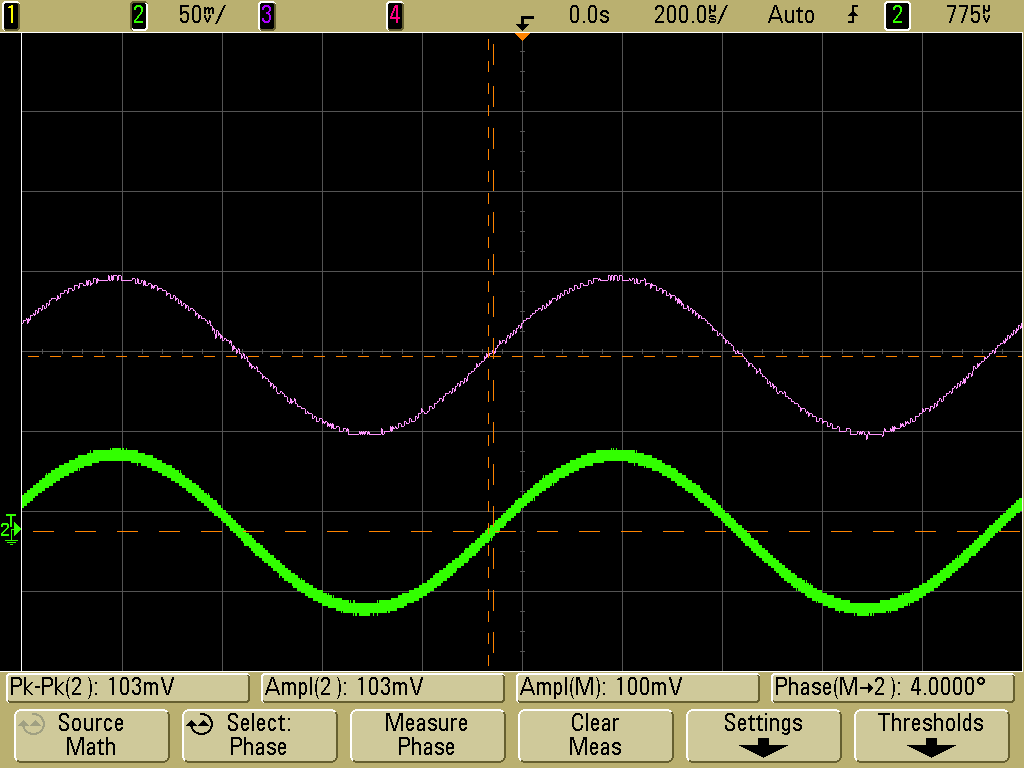
\includegraphics[scale=0.15]{./img/1c_Widerstand.png}
    \end{center}
\end{figure}
\begin{center}
\begin{tabular}{c|| c | c | c}
    & $I$ & $U$ & $\varphi$ \\
    \hline
    Kondensator ($100nF$)& $113 \mu A$ & $167mV$ & $-87^{\circ}$ \\
    Spule ($100mH$)& $139 \mu A$ & $95 mV$ & $72^{\circ}$  \\
    Widerstand ($1k\Omega$)& $104 \mu A$ & $100 mV$ & $4^{\circ}$
\end{tabular}
\end{center}
\end{frame}
\begin{frame}
\frametitle{Aufgabe 1}
\framesubtitle{Auswertung}
\begin{itemize}
    \item Komplexer Widerstand: $Z = \frac{U}{I} \left( \cos (\varphi) + i \sin
    (\varphi) \right) $
\end{itemize}
\begin{center}
\begin{tabular}{c|c|c}
    &   Messwert &  Theorie \\
    \hline
    $Z_C$ & $77.35 - i1475.85$ \Omega& $-i1592 \Omega$\\
    $Z_L$ & $211.20 + i650.00$ \Omega& $i629\Omega$ \\
    $Z_R$ & $968.51 - i 67.72$ \Omega& $1k\Omega$
\end{tabular}
\end{center}
\pause
\begin{itemize}
    \item $C = -i \frac{1}{2\pi f Z_C}$ und $L = \frac{Z_L}{i2\pi f}$:
\end{itemize}
\begin{align*}
    C &\approx 108 - i5.64nF \\
    L &\approx 103.45 - i33.61 mH
\end{align*}
\end{frame}
\begin{frame}
\frametitle{Aufgabe 1}
\framesubtitle{Auswertung}
\begin{center}
    \begin{tabular}{c|c|c}
        & Theorie & Messung \\
        \hline
        $\varphi_C$ & $-90^{\circ}$ & $-87^{\circ} $\\
        $\varphi_L$ & $90^{\circ}$ & $72^{\circ} $\\
        $\varphi_R$ & $0^{\circ}$ & $4^{\circ} $
    \end{tabular}
\end{center}
\begin{itemize}
    \item Gründe für Abweichung:
    \begin{itemize}
        \item ohmscher Widerstand der Bauteile
        \item Widerstand in Messgeräten
        \item Messungenauigkeit
    \end{itemize}
\end{itemize}
\end{frame}

\section{Analog-zu-Digital-Wandler (ADC)} % (fold)
\label{sec:Analog-zu-Digital-Wandler_(ADC}

\subsection{Erster Funktionstest} % (fold)
\label{sub:Erster Funktionstest}
\begin{frame}
\frametitle{Testsignalschaltung}
\framesubtitle{}
\begin{columns}[c]
    \column{0.65\textwidth}
         \begin{block}{$U_{in}$}
             \begin{itemize}
                \item $U_{in}$ liegt an Tiefpass:
                    \begin{equation*}
                        U_{in} = \frac{1}{\sqrt{\left(1+(R 2 \pi f
                        C)^2\right)}}\cdot U_{Fg} = 0.892V
                    \end{equation*}
                     für $f = 777Hz$,$U_{Fg} = 1V$
             \end{itemize}
         \end{block}
    \column{0.4\textwidth}
        \begin{figure}[H]
        \begin{center}
                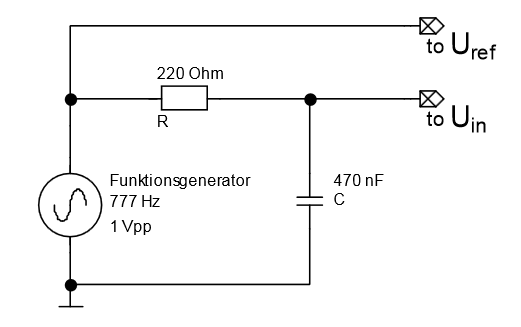
\includegraphics[scale=0.3]{./img/schaltung/testsignal.png}
        \end{center}
        \end{figure}
        \begin{figure}[H]
        \begin{center}
                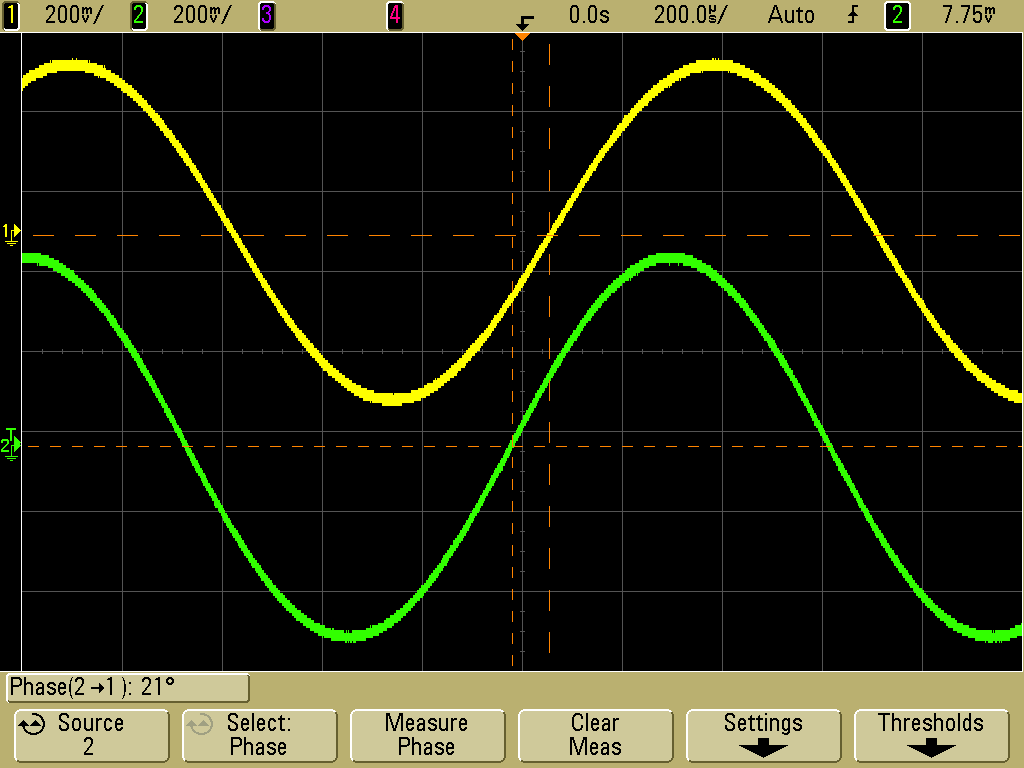
\includegraphics[scale=0.1]{./img/oszi/scope_21.png}
        \end{center}
        \end{figure}
        
        
\end{columns}

\end{frame}

\begin{frame}
\frametitle{Testsignalschaltung}
\framesubtitle{}
\begin{columns}[c]
    \column{0.65\textwidth}
         \begin{block}{Phase}
                 \begin{itemize}
                     \item Theoretische Phasenverschiebung:
                         \begin{equation*}
                             \varphi_{Th} = -\arctan{\left(2\pi f C R\right)} = 26.78^{\circ} 
                         \end{equation*}
                             für $f = 777Hz$
                    \item Gemessene Phasenverschiebung:
                        \begin{equation*}
                            \varphi_{Ge} = 21^{\circ}
                        \end{equation*}
                    \item
                        Mit $R_{Poti} = 6.96k\Omega$ bei maximalem $U_{out}$
                        ergibt sich eine Phasenverschiebung
                        \begin{equation*}
                            \varphi = 17.71^{\circ}
                        \end{equation*}
                 \end{itemize}
         \end{block}
    \column{0.4\textwidth}
        \begin{figure}[H]
        \begin{center}
                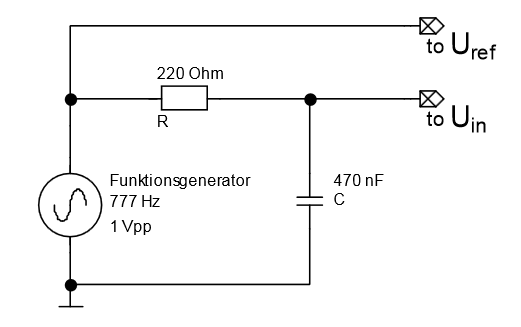
\includegraphics[scale=0.3]{./img/schaltung/testsignal.png}
        \end{center}
        \end{figure}
        \begin{figure}[H]
        \begin{center}
                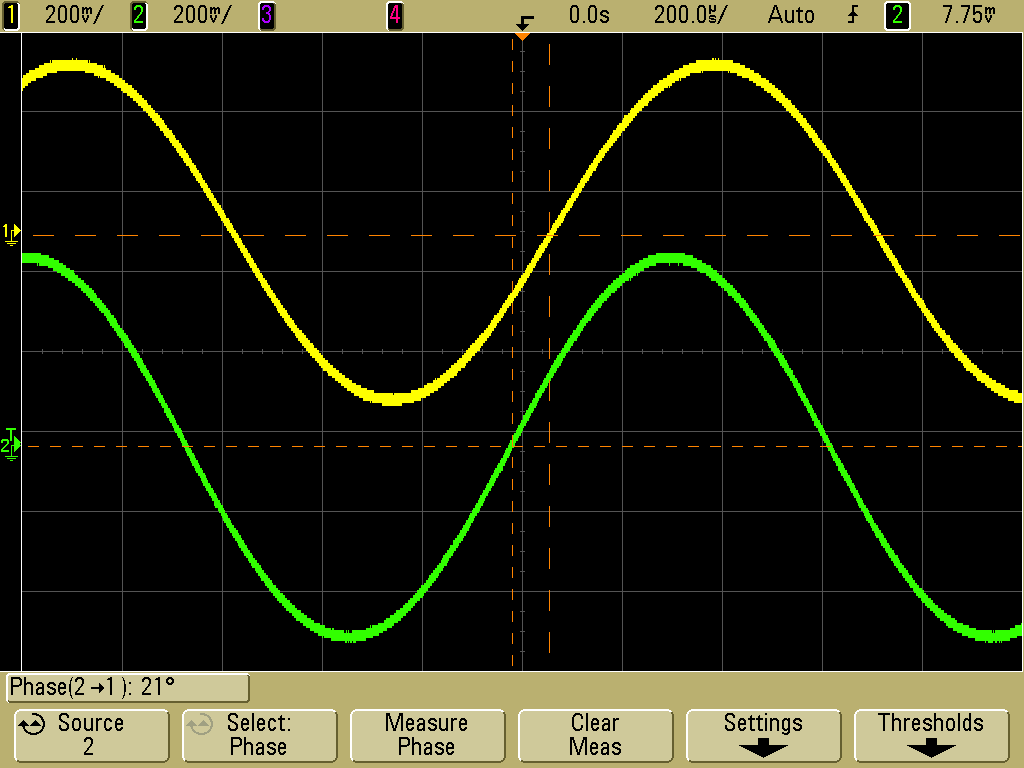
\includegraphics[scale=0.1]{./img/oszi/scope_21.png}
        \end{center}
        \end{figure}
\end{columns}
\end{frame}

\begin{frame}
    \frametitle{Messung}
    \framesubtitle{}
     \begin{figure}[H]
     \begin{center}
             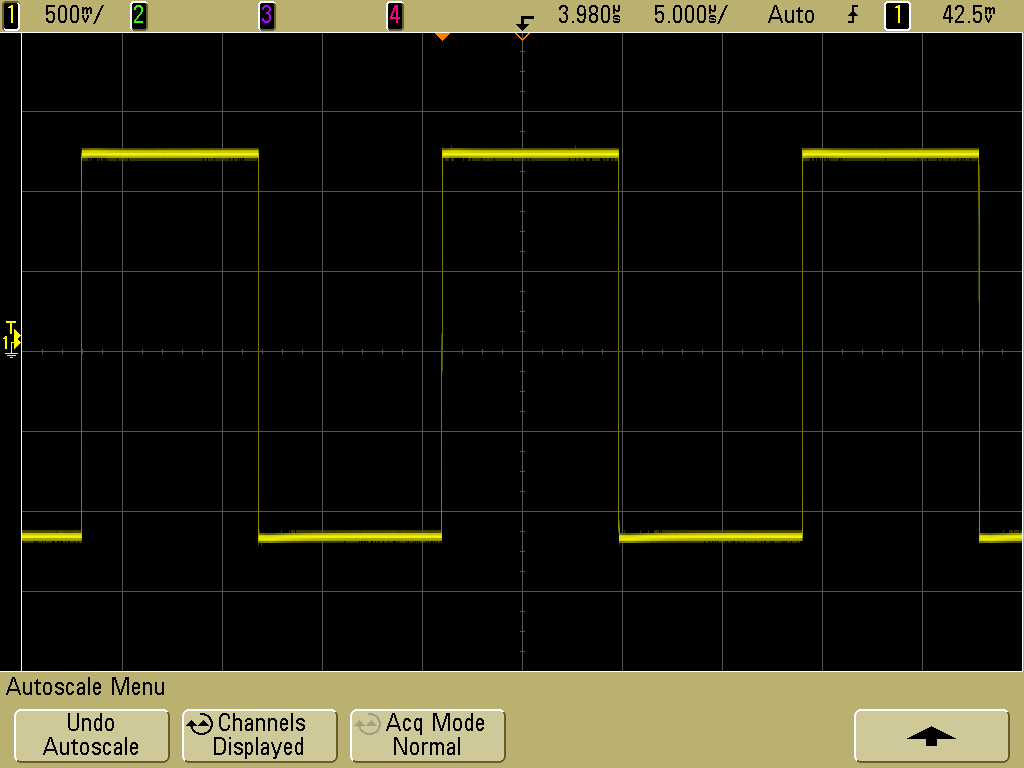
\includegraphics[scale=0.2]{./img/oszi/scope_18.png}
     \end{center}
     \caption{$U_{in}$ und $U_{ref}$ Phasenverschoben}
     \end{figure}
\end{frame}
\begin{frame}
    \frametitle{Messung}
    \framesubtitle{}
    \begin{figure}[H]
    \begin{center}
            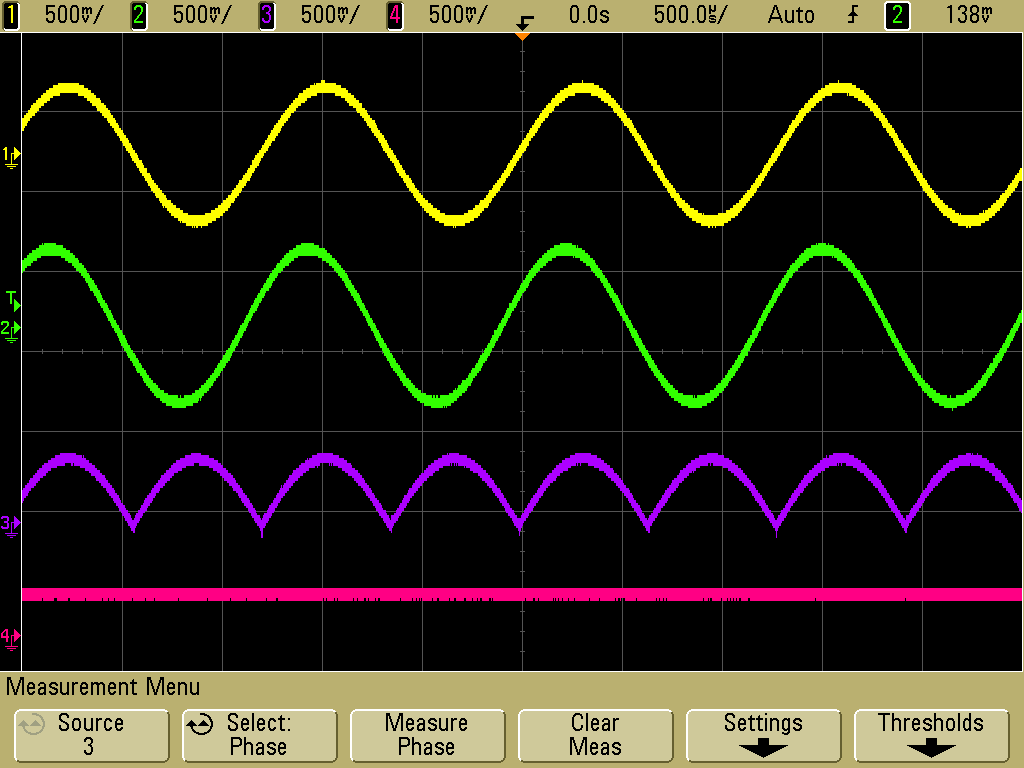
\includegraphics[scale=0.2]{./img/oszi/scope_17.png}
    \end{center}
     \caption{$U_{in}$ und $U_{ref}$ gleichphasig}
    \end{figure}
\end{frame}
% subsection Erster Funktionstest (end)

\subsection{Übertragung eines Lichtsignals} % (fold)
\label{sub:Übertragung eines Lichtsignals}
\begin{frame}
    \frametitle{Übertragung eines Lichtsignals}
    \framesubtitle{}
     \begin{columns}[c]
         \column{0.6\textwidth}
        \begin{block}{Ziel:}
             \begin{itemize}
                 \item Filterung der Störungen durch
                 \begin{itemize}
                     \item Lampen
                     \item Tageslicht
                 \end{itemize}
             \end{itemize}
        \end{block}
        \begin{block}{Versuch}
            \begin{itemize}
                \item moduliere LED-Signal mit $777Hz$ Spannung
                \item gebe Modulationsfrequenz als Referenzfrequenz weiter
                \item benutze L-I-Verstärker um $777Hz$ herauszufiltern
            \end{itemize}
        \end{block}
         \column{0.4\textwidth}
         \begin{figure}[H]
         \begin{center}
                 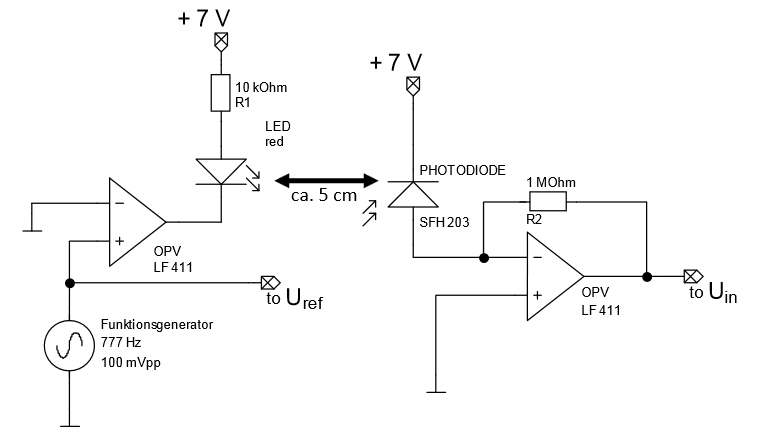
\includegraphics[scale=0.25]{./img/schaltung/optisch.png}
         \end{center}
         \end{figure}
     \end{columns}
\end{frame}

\begin{frame}
    \frametitle{Vergleich mit/ohne Abdeckung}
    \framesubtitle{}
    \begin{columns}[c]
        \column{0.5\textwidth}
        \begin{figure}[H]
        \begin{center}
                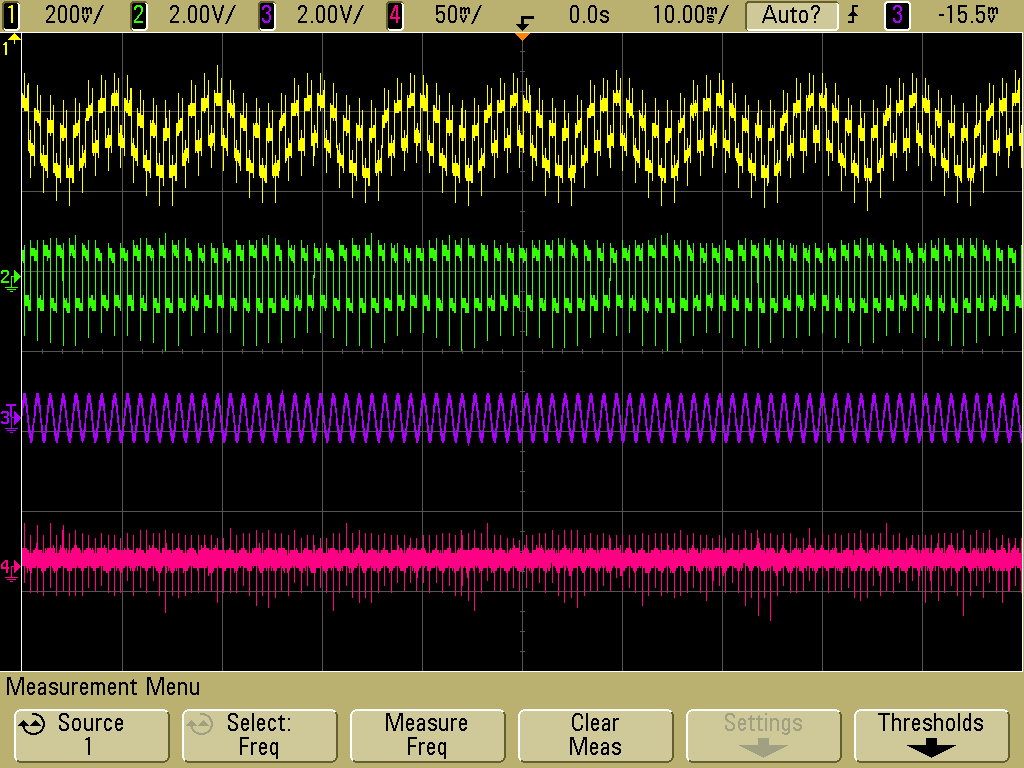
\includegraphics[scale=0.15]{./img/oszi/scope_23.png}
        \end{center}
        \caption{Ohne Abdeckung}
        \end{figure}
        \column{0.5\textwidth}
        \begin{figure}[H]
        \begin{center}
                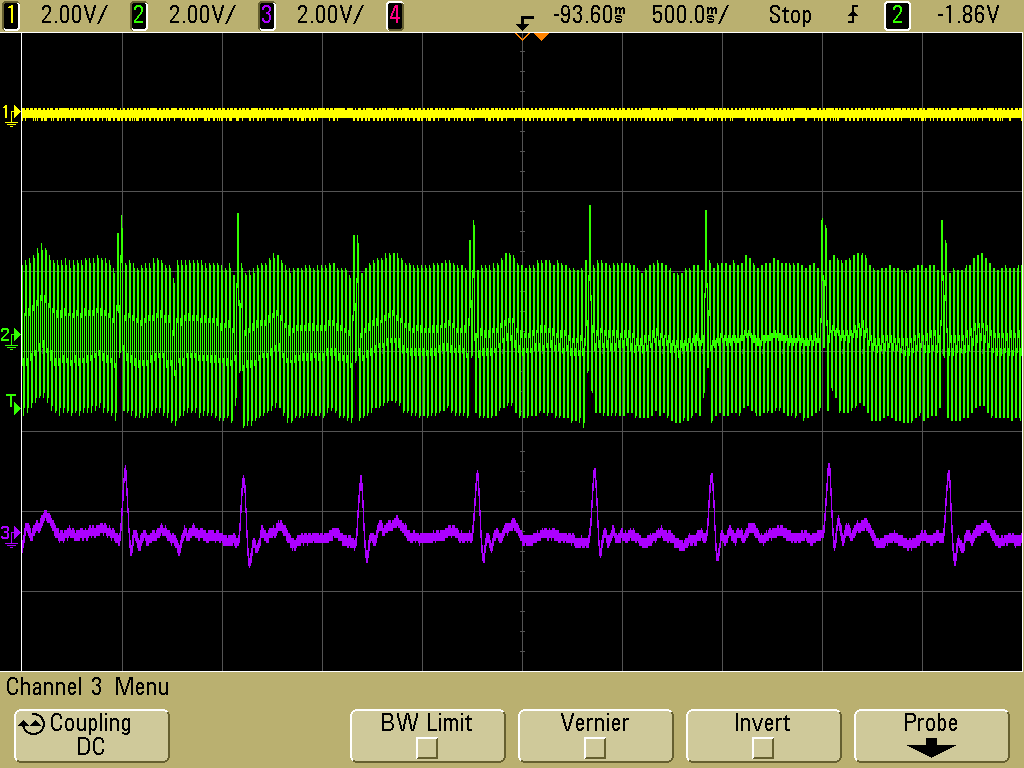
\includegraphics[scale=0.15]{./img/oszi/scope_22.png}
        \end{center}
        \caption{Mit Abdeckung}
        \end{figure}
    \end{columns}
        \begin{block}{}
            Ausgangssignal bleibt konstant auf $52.6mV$ $\rightarrow$ Schaltung
            filtert Störsignale heraus
        \end{block}
\end{frame}
% subsection Übertragung eines Lichtsignals (end)

% section Analog-zu-Digital-Wandler (ADC (end)

\begin{frame}
\frametitle{Aufgabe 4}
\framesubtitle{}
    \begin{itemize}
        \item Durch kompliziertere Schaltungen können schärfere
        Frequenztrennungen erreicht werden
        \item Beim Tiefpass wurde fälschlicherweise eine Spule mit $L=100mH$
        verwendet
    \end{itemize}
\end{frame}
\begin{frame}
\frametitle{Aufgabe 4}
\framesubtitle{Tiefpass 2. Ordnung}
\begin{figure}[H]
\begin{center}
        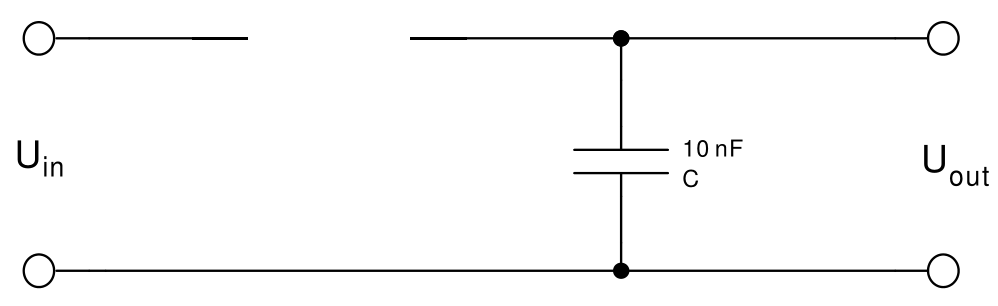
\includegraphics[scale=0.2]{./img/4a_tiefpass_1.png}
\end{center}
\end{figure}
\end{frame}
\begin{frame}
\frametitle{Aufgabe 4}
\framesubtitle{Tiefpass 2.Ordnung}
\begin{figure}[H]
\begin{center}
        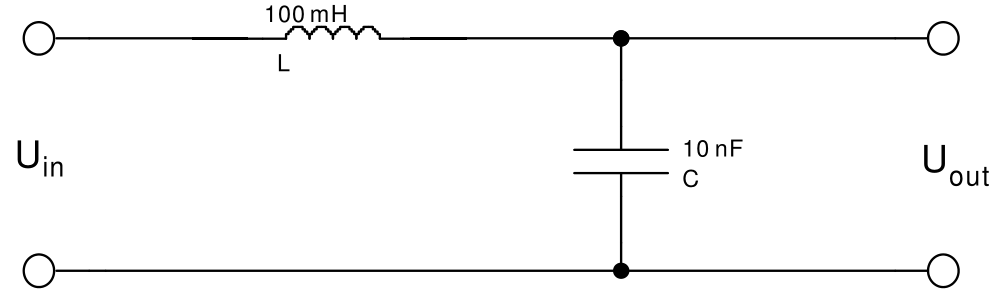
\includegraphics[scale=0.2]{./img/4a_tiefpass_2.png}
\end{center}
\end{figure}
\begin{itemize}
    \item Einbau von Spule
    \item Erwarteter Verlauf
\end{itemize}
\begin{equation*}
    \frac{U_{out}}{U_{in}} = \frac{1}{1-\omega^2 L C}
\end{equation*}
\end{frame}
\begin{frame}
\frametitle{Aufgabe 4}
\framesubtitle{Tiefpass Bode-Diagram}
    \begin{figure}[H]
    \begin{center}
            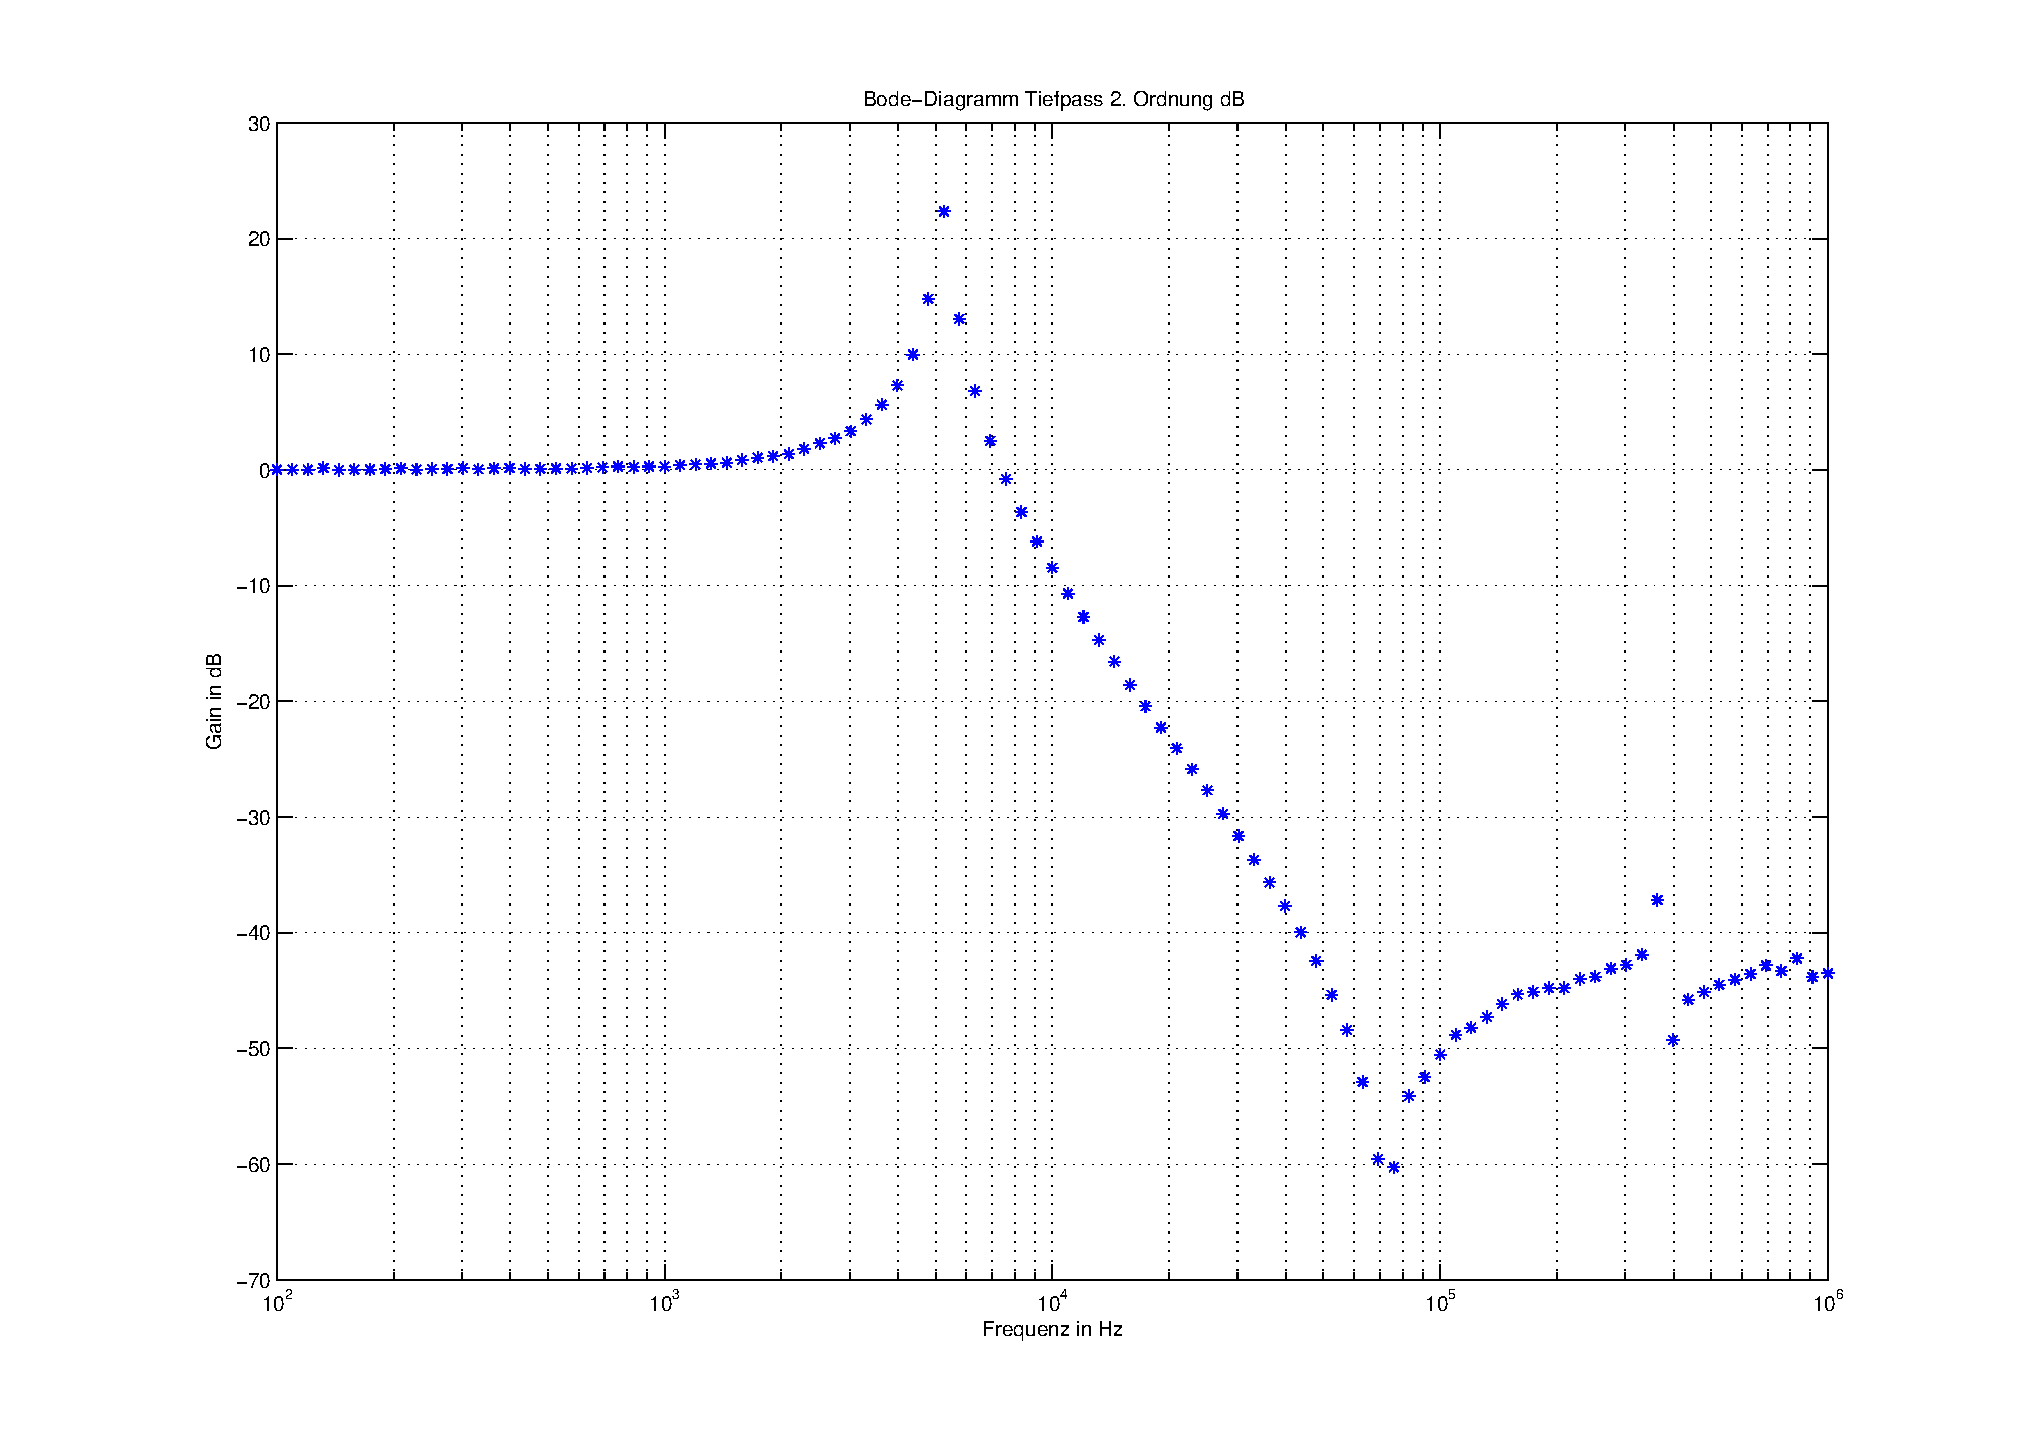
\includegraphics[scale=0.50]{./img/4a_bode_tief_dB.eps}
    \end{center}
    \end{figure}  
\begin{itemize}
    \item Unerwünschte Asymptote bei $\omega = \sqrt{\frac{1}{LC}}$
    \item Schwinkreis ohne Dämpfung
\end{itemize}
\end{frame}
\begin{frame}
    \frametitle{Aufgabe 4}
    \framesubtitle{Tiefpass mit Widerstand}
     %\begin{figure}[H]
     %\begin{center}
     %        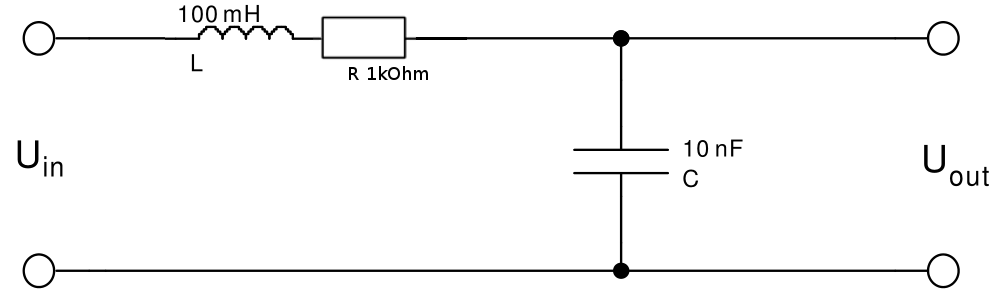
\includegraphics[scale=0.2]{4a_tiefpass_3.png}
     %\end{center}
     %\end{figure} 
     \begin{itemize}
        \item Zusätzlicher Widerstand
         \item Erwarteter Verlauf
     \end{itemize}
     \begin{equation*}
         \frac{U_{out}}{U_{in}}
         =
         \frac{Z_C}{Z_C + Z_L + R}
         =
         \frac{1}{\sqrt{\omega^4 L^2 C^2 + \omega^2 R^2 C^2 - 2 \omega^2 LC + 1}}
     \end{equation*}
\end{frame}
\begin{frame}
    \frametitle{Aufgabe 4}
    \framesubtitle{Tiefpass mit Widerstand}
     \begin{figure}[H]
     \begin{center}
             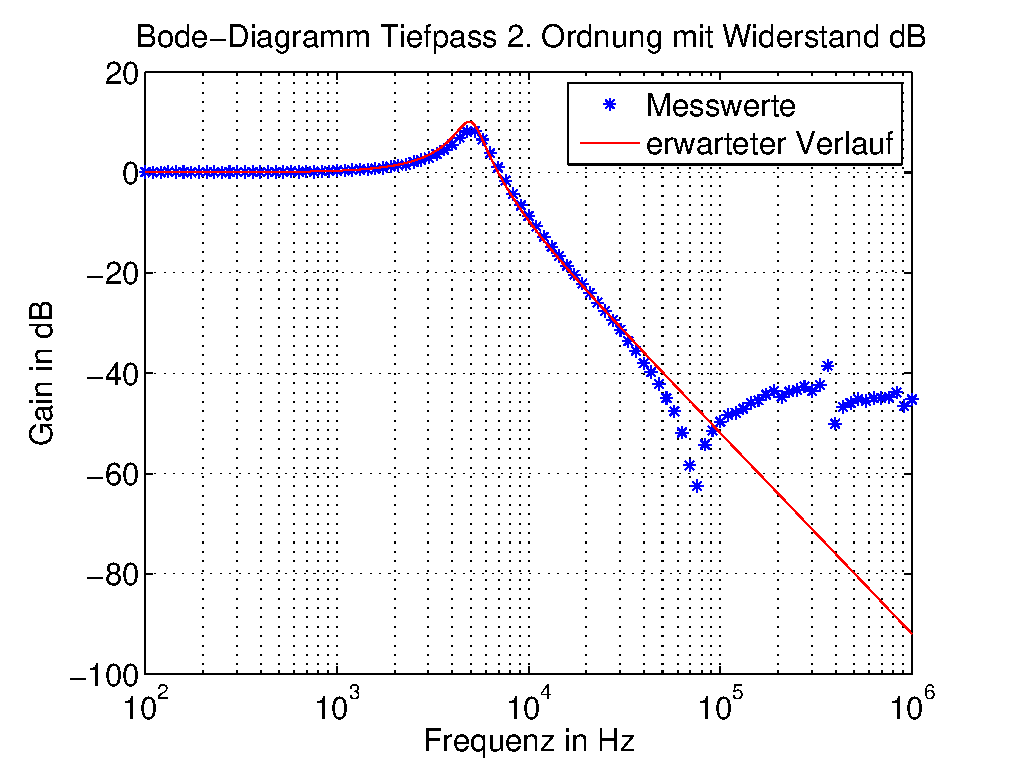
\includegraphics[scale=0.45]{./img/4a_bode_tief_dB_W.eps}
     \end{center}
     \end{figure}
     \begin{itemize}
        \item keine Asymptote
         \item Peak vor Abfall ist deutlich kleiner
         \item $R$ dämpft den Schwingkreis
     \end{itemize}
\end{frame}
\begin{frame}
    \frametitle{Aufgabe 4}
    \framesubtitle{Sperrkreisfilter}
    \begin{figure}[H]
    \begin{center}
            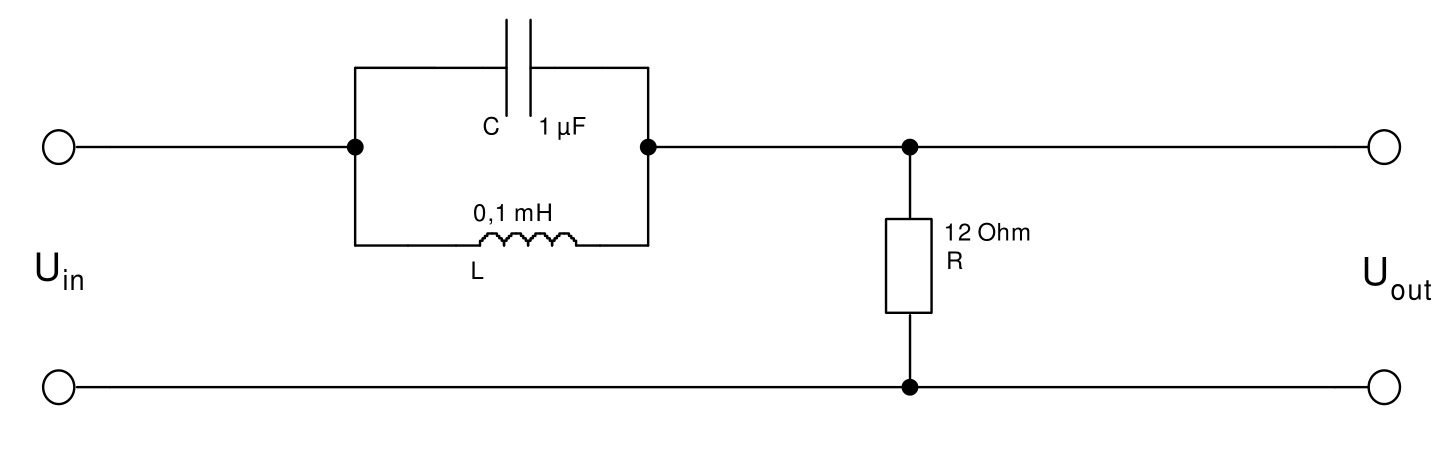
\includegraphics[scale=0.2]{./img/4b_schaltung.png}
    \end{center}
    \end{figure}
    \begin{equation*}
        \frac{U_{out}}{U_{in}}
        =
        \frac{\left\vert Z_R \right\vert}{\left\vert \frac{1}{\frac{1}{Z_C}+\frac{1}{Z_L}}
        +Z_R \right\vert }
        =
        \frac{R}{\sqrt{\left(\frac{\omega L}{\omega^2 C L +1}\right)^2 +
        R^2}}
    \end{equation*}
\end{frame}
\begin{frame}
    \frametitle{Aufgabe 4}
    \framesubtitle{Bode-Diagramm Sperrkreisfilter}
     \begin{figure}[H]
     \begin{center}
             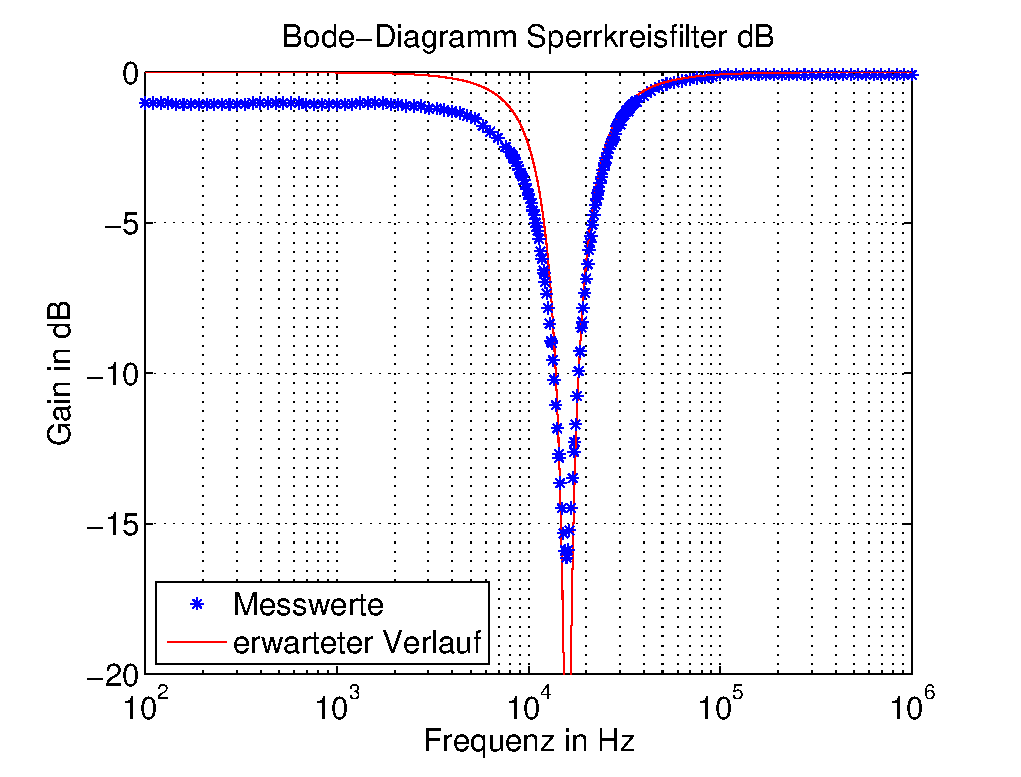
\includegraphics[scale=0.55]{./img/4b_dB.eps}
     \end{center}
     \end{figure}
\end{frame}
\begin{frame}
    \frametitle{Aufgabe 4}
    \framesubtitle{Bode-Diagramm Sperrkreisfilter}
     \begin{figure}[H]
     \begin{center}
             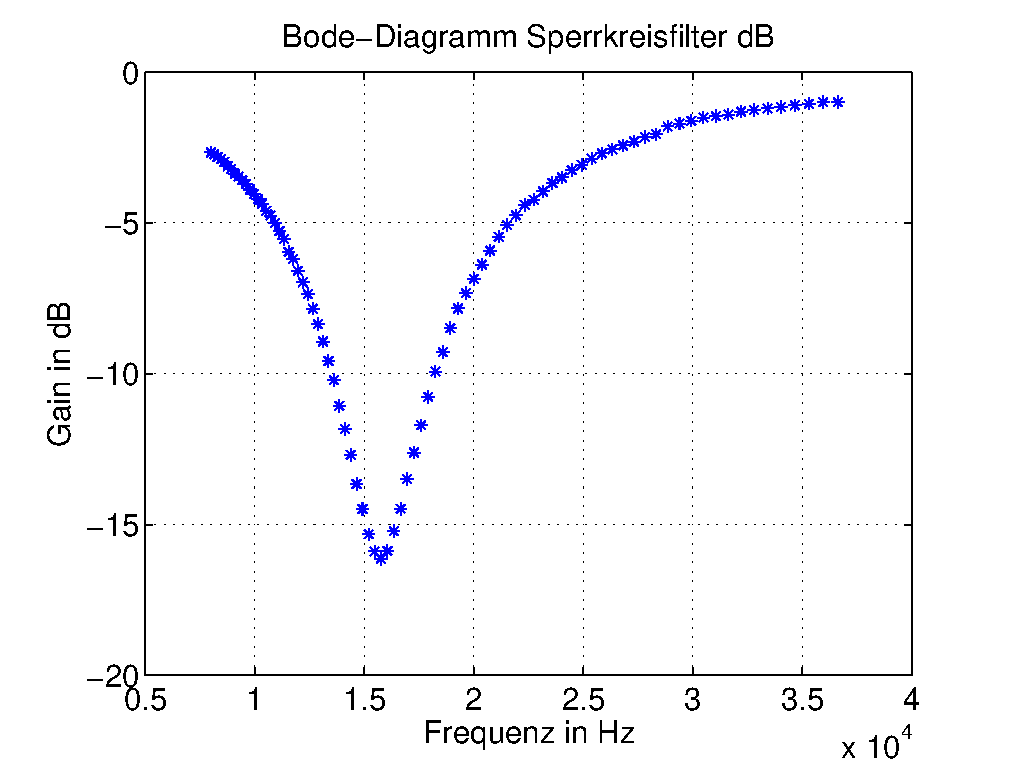
\includegraphics[scale=0.45]{./img/4b_Peak.eps}
     \end{center}
     \end{figure}
    \begin{itemize}
        \item Filtert einzelne Frequenz raus: $f \approx 16 kHz$
        \item Theorie: $f= \frac{1}{2\pi \sqrt{LC}}=15.91kHz$
    \end{itemize}
\end{frame}
\begin{frame}
    \frametitle{Aufgabe 4}
    \framesubtitle{Bode-Diagramm Sperrkreisfilter Phase}
     \begin{figure}[H]
     \begin{center}
             \includegraphics[scale=0.55]{./img/4b_Phase.eps}
     \end{center}
     \end{figure}
     \begin{itemize}
         \item Phase dreht sich beim Peak um
     \end{itemize}
\end{frame}

%\chapter{Masse, Größe und Struktur der Atome} % (fold)
\label{cha:Masse,_Groesse_und_Struktur_der_Atome}
\section{Wellenfunktion, Schrödingergleichung und die Postulate der
Quantenmechanik} % (fold)
\label{sec:Wellenfunktion,_Schrödingergleichung_und_die_Postulate_der_Quantenmech}
\subsubsection{1. Postulat (Wellenfunktion, Zustand)} % (fold)
\label{ssub:1._Postulat_(Wellenfunktion,_Zustand)}
Der Zustand eines \qmn Systems wird durch eine Wellenfunktion
(Zustandsfunktion/Zustand) $\Psi$ beschrieben, die i.A von den Koordinaten
aller Teilchen un der Zeit abhängt.

Z.B ein Teilchen $\vec{r}=(x,y,z) \quad \Psi(x,y,z,t)= \Psi(\vec{x},t)$

Die Wahrscheinlichkeit das Teilchen (zur Zeit $t$) im Bereich $V \in
\mathbb{R}^3$ zu finden ist gegeben durch
\begin{equation*}
    \int_V d^3 r \lv \Psi(\vec{r},t)\rv^2
\end{equation*}

Für infinitesimale Volumen $dV$ ist $\lv \Psi(\vec{r},t)\rv^2 dV$ die
Wahrscheinlichkeit das Teilchen in $dV$ um $\vec{r}$ zu finden.
    
$\varphi(\vec{r},t) = \lv \Psi(\vec{r},t)\rv^2$ ist die Wahrscheinlichkeitsdichte.

Es gilt die Normierungsbedingung
\begin{equation*}
    \int_{\mathbb{R}^3} d^3 r \lv \Psi(\vec{r},t)\rv^2=1
\end{equation*}
fall $\Psi$ quadratintegrabel.
\begin{bem}
    \item 
    Systeme mit $n$ Teilchen $\vec{r}_j = (x_j),y_j,z_j) \quad j=1 \ldots
    n \rightarrow \Psi(\vec{r}_1, \ldots, \vec{r}_n,t)$

    $H_2$ Molekül (2 Elektronen, 2 Protonen): $\Psi(r_1,r_2,r_3,r_4,t)$ 
    \item
    i.A $\Psi(\vec{r},t) \in \mathbb{C}$
    \item
    $\Psi$ ist bist auf globalen Phasenfaktor eindeutig 
    \begin{align*}
        \tilde{\Psi}(\vec{r},t)=
        e^{ia} \Psi(\vec{r},t) \\
        \tilde{\varphi}=\lv \tilde{\Psi} \rv^2 = \lv \Psi \rv^2 = \varphi
    \end{align*}
    \item Mathe: $\Psi \in W$, $W$ Vektorraum (Hilbertraum)

    Es gilt Superpositionsprinzip: $\Psi_1, \Psi_2 \in W$ mögliche
    Systemzustände, dann auch $c_1 \Psi_1 + c_2 \Psi_2 \in W$, $c_1,c_2 \in
    \mathbb{C}$. 

    Betrachte Teilchen mit Masse $m$, Geschwindigkeit $v$:
    %Bild

    Mit
    $k=\frac{2\pi}{\lambda},\lambda=\frac{h}{mv},k=\frac{mv}{\frac{h}{2\pi}}$
    folgt
    \begin{equation*}
        e^{ikz} = e^{\frac{i}{\hbar}mvz}
    \end{equation*}
    Rechts:
    \begin{align*}
        \Psi(x) &= \Psi_1(x) + \Psi_2(x) \\
        \Psi_{1/2}(x) &= n e^{\frac{imv}{2\hbar L}\left(x \pm \frac{d}{2}\right)^2} \\
        &= n e^{\frac{imv}{2\hbar L}\left(x^2 + \frac{d}{r}\right)} \
        e^{\pm \frac{imvxd}{2\hbar L}}
    \end{align*}
    Intensität am Schirm $\sim \varphi(x)$:
    \begin{align*}
       \varphi(x) &= \lv \Psi(x) \rv^2 = \lv \Psi_1(x) + \Psi_2(x)\lv^2 \\
                &= \lv \Psi_1(x) \rv^2 + \lv \Psi_2(x) \rv^2 \
                    + 2\Re \left( \Psi_1(x) \Psi_2^*(x) \right) \\
                &= \lv n \rv^2  \left( 1 + 1 + 2\Re \left( e^{-2i \
                    \frac{mvxd}{2\hbar L}}\right) \right)\\
                &= 2 \lv m \rv^2 \left( 1 + \cos \left(\frac{mvd}{\hbar L}x \right) \right)
    \end{align*}
    \item \qme Wahrscheinlichtkeitsbeschreibung
    \begin{equation*}
        \varphi(\vec{r},t) = \lv \Psi(\vec{r},t)\rv^2
    \end{equation*}
    Aussage über eine Vielzahl von Messungen an identischen Systemen.

    $\longrightarrow$ Indeterminisums
\end{bem}
Benis
banis
bonis
% subsubsection 1. Postulate (Wellenfkt, Zustand) (end)
% section Wellenfunktion, Schrödingergleichung und die Postulate der Quantenmech (end)

\section{Impulsoperator, Impulseigenfunktion, Impulsraumdarstellung} % (fold)
\label{sec:Impulsoperator,_Impulseigenfunktion,_Impulsraumdarstellung}
\begin{equation*}
    \h{p_x} = \frac{\hbar}{i} \frac{\p}{\p }
\end{equation*}
\begin{equation*}
    \h{\vec{p}}=\frac{\hbar}{i} \vec{\nb}
\end{equation*}
\subsection{Konsistenz der Definition} % (fold)
\label{sub:Konsistenz_der_Definition}
klassiche Mechanik $p=mv=m \frac{d v}{d t}$
Betrachte Bewegungsgleichung für Mittelwert
\begin{equation*}
    \frac{d }{d }\left\langle \h{x} \right\rangle (t) 
    =
    \frac{d }{d }
\end{equation*}
% subsection Konsistenz der Definition (end)
\subsection{Wahrscheinlichkeitsstromdichte mit Kontinuitätsgleichung} % (fold)
\label{sub:Wahrscheinlichkeitsstromdichte_mit_Kontinuitätsgleichung}
\begin{gather*}
     \varphi = \lv \Psi(r,t)\rv^2 \\
     \frac{\p}{\p t} \varphi(\vec{r},t) = \frac{\p}{\p t} \Psi^*(\vec{r},t)
     \Psi(r,t) = \frac{\p \Psi^*}{\p t} \Psi + \Psi^* \frac{\p \Psi}{\p t}
\end{gather*}
\begin{align*}
    i \hb \frac{\p \Psi}{\p t} 
    &= 
    - \frac{\hbar^2}{2m} \Delta \Psi + \nb \Psi \\
    - i \hb \frac{\p \Psi^*}{\p t}
    &=
    - \frac{\hb^2}{2m} \Delta \Psi^* + \nb \Psi^*
\end{align*}
\begin{align*}
    \frac{\p}{\p t} \varphi
    &=
    \frac{1}{-i\hb} \left[ - \frac{\hb^2}{2m} \Delta \Psi^* + \nb \Psi^*\right] \Psi 
    + \Psi^* \frac{1}{i\hb} \left[ - \frac{\hb^2}{2m} \Delta \Psi + \nb
    \Psi \right] \\
    &=
    \frac{\hb}{2m} \left[ \lk \Delta \Psi^* \rk \Psi - \Psi^* \lk \Delta \Psi
    \rk \right] \\
    &=
    \frac{\hb}{2m} \vec{\nb} \cd \left[ \lk \vec{\nb} \Psi^* \rk \Psi -
    \Psi^* \vec{\nb} \Psi \right]
\end{align*}
\begin{align*}
    \frac{\p}{\p t} \varphi(\vec{r},t) + \vec{\nb} \cd 
    \underbrace{\frac{\hb}{2m}\left[\Psi^*(\vec{\nb} \Psi) - \Psi(\vec{\nb}
    \Psi^*) \right] }_{\vec{j}(\vec{r},t) \quad
    \text{Wahrscheinlichkeitsstrom}}&= 0 \\
    \frac{d }{d t} \varphi(\vec{r},t) + \vec{\nb} \cd \vec{j}(\vec{r},t) &= 0
\end{align*}
Betrachte Bewegungsgleichung für Mittelwert:
\begin{align*}
     \frac{d }{dt} \left\langle \h{x} \right\rangle (t)
     &= \frac{d }{d t} \int dx \Psi^*(x,t) \h{x} \Psi(x,t)
     = \frac{d }{d t} \int dx  \Psi^*(x,t) x \Psi(x,t) \\
     &=
     \int dx \lk 
     \underbrace{\frac{\p \Psi^*}{\p t} x \Psi}_{\frac{1}{ \lk -i \hb \rk }
     \lk -\frac{\hb^2}{2m} \frac{\p \Psi^*}{\p x^2} + \nabla \Psi^* \rk }
     + 
     \underbrace{\Psi^* x \frac{\p \Psi}{\p t}}_{\frac{1}{ \lk i \hb \rk } 
     \lk -\frac{\hb^2}{2m} \frac{\p^2 \Psi}{\p x^2} + \nabla \Psi \rk }
     \rk \\
     &=
     \frac{\hb}{2im} \int dx \lk \frac{\p^2 \Psi^*}{\p x^2}x \Psi 
     - \Psi^* x \frac{\p^2 \Psi}{\p x^2} \rk  \\
\end{align*}
\begin{eins}{NR:}
     \begin{align*}
         \int dx \frac{\p^2 \Psi^*}{\p x^2} x \Psi
         &\underset{PI}{=}
         \int dx \Psi^* 
         \underbrace{ \frac{\p^2}{\p x^2}\lk x \Psi \rk}_{\frac{\p}{\p x}\lk -
         \Psi + x \frac{\p^2 \Psi}{\p x^2}\rk  = 2 \frac{\p \Psi}{\p x} + x
         \frac{\p^2 \Psi}{\p x^2}}
     \end{align*}
     Randerterme verschwinden: $\Psi(x) \underset{x \pm \infty}{\rar} 0$.
\end{eins}
\begin{align*}
     &=
     \frac{\hb}{2im} \int dx \lk 2 \Psi^* \frac{\p\Psi}{\p x}
     + \Psi^* x \frac{\p^2 \Psi}{\p x^2}
     - \Psi^* x \frac{\p^2 \Psi}{\p x^2} \rk \\
     &=
     \frac{1}{m} \int dx \Psi^*(x,t) \underbrace{\frac{\hb}{i} \frac{\p}{\p
     x}}_{= \h{p}_x} \Psi(x,t) \\
     &=
     \frac{1}{m} \int dx \Psi^* \h{p}_x \Psi \\
     &=
     \frac{1}{m} \left\langle \h{p}_x \right\rangle (t)
     =
     \frac{d }{d t} \left\langle \h{x} \right\rangle (t)
     \rar \text{genau wie klassische Mechanik}
\end{align*}
% subsection Wahrscheinlichkeitsstromdichte mit Kontinuitätsgleichung (end)
\subsection{Impulsoperator: Generator für Translation} % (fold)
\label{sub:Impulsoperator:_Generator_für_Translation}
\begin{align*}
    e^{a \frac{\p}{\p x}} \Psi(x)
    &=
    \underbrace{\sum_{n=0}^\infty \frac{a^n}{n!} \frac{\p^n}{\p x^n} \Psi \quad a \in
    \mathbb{R}}_{\text{Taylorentwicklung}} \\
    &=
    \Psi(x+a)
\end{align*}
Impulsoperator $\h{p}_x = \frac{\hb}{i} \frac{\p}{\p x}$:
\begin{equation*}
    e^{\frac{i}{\hb} a \h{p}_x} \Psi(x) =
    e^{a \frac{\p}{\p x}} \Psi(x) = \Psi(x+a)
\end{equation*}
% subsection Impulsoperator: Generator für Translation (end)
\subsection{Impulseigenschaften} % (fold)
\label{sub:Impulseigenschaften}
\begin{align*}
    \h{p} \varphi(x) &= p' \varphi(x) \quad a \in \mathbb{R}\\
    \frac{\hb}{i} \frac{d }{d x} \varphi(x) &= p' \varphi(x) \\
\end{align*}
\begin{equation*}
    \tag*{\text{(verallgemeinerte Eigenfunktion)}}
    \rar
    \boxed{
        \varphi_{p'}(x) = c e^{\frac{i}{\hb} p' x}
    }
    \quad p' \in \mathbb{R} 
\end{equation*}
$\varphi_{p'}(x)$ nicht normierbar: $\int_{-\infty}^{\infty} \lv \varphi_{p'}
\rv^2 = \infty$.

Konvention zur Festsetzung von $c$:
\begin{align*}
    \delta(p_1 - p_2) \overset{!}{=} \int dx \varphi_{p'}^*(x) \varphi_{p_2}(x)
    &=
    \underbrace{\lv c \rv^2 \int_{-\infty}^{\infty} e^{- \frac{i}{\hb} p_1 x}
    e^{\frac{i}{\hb}  p_2 x}}_{=\int_{-\infty}^{\infty} dx e^{\frac{i}{\hb} x \lk
    p_2 - p_1 \rk} = 2 \pi \hbar \delta (p_1 - p_2)} \\
    &=
    \lv c^2 \rv 2 \pi \delta(p_1 - p_2) 
\end{align*}
\begin{equation*}
    \rar c= \frac{1}{\sqrt{2\pi\hb}}
\end{equation*}
\begin{equation*}
    \varphi_{p_1}(x) = \frac{1}{\sqrt{2 \pi \hb}} e^{\frac{i}{\hb} p'_x}
\end{equation*}
System im Zustand $\Psi$: Wahrscheinlichkeit den Impuls $p'$ zu messen:
\begin{align*}
    W(p')
    &=
    \lv \int_{-\infty}^{\infty} dx \Psi_{p'}^*(x) \Psi(x) \rv^2 \\
    &=
    \underbrace{\lv \frac{1}{\sqrt{2\pi\hb}} 
    \int_{-\infty}^{\infty} dx e^{-\frac{i}{\hb}p'x}\Psi(x)
    \rv^2}_{\text{Fourriertransformierte} = \tilde{\Psi}(p')} \\
    &=
    \underbrace{\lv \tilde{\Psi}(p')\rv^2}_{\text{Wahrscheinlichkeitsdichte}}
\end{align*}
denn
\begin{align*}
    \int_{-\infty}^{\infty} dp' W(p')
    &=
    \int_{-\infty}^{\infty} dp' \tilde{\Psi}^*(p') \tilde{\Psi}(p') \\
    &=
    \int_{-\infty}^{\infty} dp' \frac{1}{\sqrt{2 \pi \hb}}
    \int dx' e^{\frac{i}{\hb} p' x'} \Psi^*(x') \\
    &=
    \frac{1}{\sqrt{2 \pi \hb}} \int_{-\infty}^{\infty} dx e^{- \frac{i}{\hb}p'
    x} \Psi(x)\\
    &=
    \int dx \int dx' \Psi^*(x)\Psi(x)
    \underbrace{\int_{-\infty}^{\infty} dp' \frac{1}{2 \pi \hb}
    e^{\frac{i}{\hb} p' \lk x' - x \rk }}_{=\delta(x-x')}\\
    &=
    \int dx \Psi^*(x)\Psi(x) = \int dx \lv \Psi(x) \rv^2 = 1
\end{align*}
\begin{eins}{Mathematisch:}
     \begin{equation*}
         \int dx \lv \Psi(x) \rv^2 = \int dp \lv \tilde{\Psi}(p) \rv^2
     \end{equation*}
     gilt generell für Fourriertransformationen $\rar$ Parsevalsches Theorem
\end{eins}
% subsection Impulseigenschaften (end)
\subsection{Impulsraumdarstellung der Wellenfunktion} % (fold)
\label{sub:Impulsraumdarstellung_der_Wellenfunktion}
$\Psi(x,t)$ Wellenfunktion im Ortsraum.
\begin{equation*}
    \tag*{\text{(Wellenfunktion im Impulsraum)}}
    \tilde{\Psi}(p,t) =
    \frac{1}{\sqrt{2 \pi \hbar}} \int dx e^{- \frac{i}{\hbar}p_x} \Psi(x,t)
\end{equation*}
% subsection Impulsraumdarstellung der Wellenfunktion (end)
\subsection{Impulsraumdarstellung von Operatoren} % (fold)
\label{sub:Impulsraumdarstellung_von_Operatoren}
$\Psi(x,t)$ Wellenfunktion im Ortsraum.
\begin{gather*}
    \h{x}\Psi(x) = x \Psi(x) \quad \h{p}\Psi(x) = \frac{\hb}{i}\frac{\p\Psi}{\p
    x} \\
    A(x,p) \rar \h{A} = A(x,\frac{h}{i} \frac{\p}{\p x} \\
    \text{konsistent mit} \qquad \left\langle \h{A}  \right\rangle =
    \int dx \Psi^*(x) \h{A} \Psi(x) \\
    \text{Berechnung von Erwartungswert:} \quad \left\langle \h{x}
    \right\rangle = \int dx \lv \Psi(x) \rv^2 x
\end{gather*}
Wirkung von Operatoren direkt im Impulsraum $\tilde{\Psi}(p,t)$:
\begin{align*}
    \left\langle \h{p} \right\rangle 
    &=
    \int dp \lv \tilde{\Psi}(p) \rv^2 p = \int dp \tilde{\Psi}^*(p)
    \underbrace{p \tilde{\Psi}(p)}_{\h{p}\tilde{\Psi}} \\
    &=
    \int dp \tilde{\Psi}^* (p) \h{p} \tilde{\Psi}(p)
\end{align*}
\begin{equation*}
    \h{p}\tilde{\Psi}(p) = p \tilde{\Psi}(p)
\end{equation*}
\begin{eins}{Fourrier-Rücktransformation}
    \begin{equation*}
        \Psi(x) = \frac{1}{\sqrt{2 \pi \hb}} \int dp e^{\frac{i}{\hb}px}
        \tilde{\Psi}(p)
    \end{equation*}
\end{eins}
\begin{align*}
    \lv \h{x} \rv 
    &=
    \int dx \Psi^*(x) x \Psi(x) \\
    &=
    \int dx \int dp \int dp' \frac{1}{2 \pi \hb} e^{-  \frac{i}{\hb} xp'}
    \tilde{\Psi}^*(p') x e^{\frac{i}{\hb} px} \tilde{\Psi}(p)
\end{align*}
\begin{einsn}
    \begin{equation*}
        x e^{\frac{i}{\hb}px}\tilde{\Psi}(p) = \tilde{\Psi}(p)
        \frac{\hb}{i}\frac{\p}{\p p}  e^{\frac{i}{\hb}px}
    \end{equation*}
\end{einsn}
\begin{align*}
    &=
    \int dp \int dp' \tilde{\Psi}^*(p')\tilde{\Psi}(p) \frac{\hb}{i}\frac{\p}{\p
    p} \underbrace{\int dx \frac{1}{2 \pi \hb} e^{\frac{i}{\hb}x \lk p-p' \rk
    }}_{\delta(p-p')}\\
    &=
    \int dp \int dp' \tilde{\Psi}^*(p)\tilde{\Psi}(p) \frac{\hb}{i}
    \frac{\p}{\p p} \delta(p - p') \\
    &=
    \int dp \int dp' \tilde{\Psi}^*(p) \lk - \frac{\hb}{i}
    \frac{\p \tilde{\Psi}}{\p p}\rk \delta(p -p') \\
    &=
    \int dp \tilde{\Psi}^*(p')\lk -  
    \underbrace{\frac{\hb}{i}\frac{\p}{\p p}}_{= \h{x}}\rk \tilde{\Psi}(p)
    =
    \left\langle \h{x} \right\rangle 
\end{align*}
Im Impulsraum $\tilde{\Psi}(p)$:
\begin{gather*}
    \h{p} \tilde{\Psi}(p) = p \tilde{\Psi}(p)\\
    \h{x} \tilde{\Psi}(p) = i\hb \frac{\p}{\p p} \tilde{\Psi}(p)\\
    A(x,p) \rar \h{A} \tilde{\Psi}(p) = A(i \hb \frac{\p}{\p p},p)
    \tilde{\Psi}(p)
\end{gather*}
% subsection Impulsraumdarstellung von Operatoren (end)
\subsection{Verallgemeinerung in $3D$} % (fold)
\label{sub:Verallgemeinerung_in_$3D$}
\begin{gather*}
    \h{\vec{p}}\Psi(\vec{r}) = \frac{\hb}{i} \vec{\nabla} \Psi(\vec{r})\\
    i = x,y,z \qquad \h{p}_i \varphi_{\vec{p'}}(\vec{r}) = p'_j
    \varphi_{\vec{p'}}(\vec{r}) \\
    \varphi_{\vec{p'}}(\vec{r}) = 
    \frac{1}{\lk 2 \pi \hb \rk^{\frac{2}{3}}} e^{\frac{i}{\hb}\vec{p'}\vec{r}}\\
    W(\vec{r}')=
    \lv \int d^3 \varphi_{\vec{p}'}^* (\vec{r}) \Psi(\vec{r}) \rv^2
    =
    \lv
    \underbrace{
    \frac{1}{\lk 2 \pi \hb \rk^{\frac{2}{3}}} \int d^3 r e^{- \frac{i}{\hb}\vec{p}\vec{r}}\Psi(\vec{r})
    }_{
    \tilde{\Psi}(\vec{p}')}
    \rv^2
\end{gather*}
% subsection Verallgemeinerung in $3D$ (end)
% section Impulsoperator, Impulseigenfunktion, Impulsraumdamrstellung (end)

\section{Das freie Teilchen - Wellenpakete} % (fold)
\label{sec:Das_freie_Teilchen_-_Wellenpakete}
Teilchen mit Masse $m$, eindimensional ohne Kräfte.
\begin{erl}{Hamiltonoperator:}
     \begin{equation*}
         \h{H}=\frac{\h{p}^2}{2m}+\underset{=0}{V(\h{x})}=\frac{\h{p}^2}{2m}= -
         \frac{\hb}{2m}\frac{\p^2}{\p x}
     \end{equation*}
\end{erl}
\begin{erl}{Schrödingergleichung}
      \begin{equation*}
          i \hb \frac{\p}{\p t} \Psi(x,t) = \h{H} \Psi(x,t) =
          -\frac{\hb^2}{2m}\frac{\p^2 \Psi}{\p x^2}
      \end{equation*}
\end{erl}
Separationsansatz $\Psi(x,t) = \varphi(x) \chi(t)$
\begin{align*}
    i \hb \varphi \frac{d \chi}{d t} &= -\frac{\hb^2}{2m} \frac{d^2
    \varphi}{dx^2 } \\
    &=
    i \hb \underbrace{\frac{1}{\chi}\frac{d x}{d t}}_{t}
    =
    - \frac{\hb^2}{2m} \underbrace{\frac{1}{\varphi} \frac{d^2
    \varphi}{dx^2}}_{x}
    = const = E
\end{align*}
\begin{gather*}
     \frac{d \chi }{dt}=- \frac{i}{\hb} E \chi \rar \chi(t) = c
     e^{-\frac{i}{\hb}E t} \\
     \underbrace{-\frac{\hb^2}{2m}\frac{d^2}{dx^2}}_{\h{H}}\varphi(x) = E \varphi(x)
\end{gather*}
\begin{equation*}
    \tag*{\text{(stationäre Schrödingergleichung)}}
    \h{H} \varphi(x) = E \varphi(x)
\end{equation*}
$\rar$ Eigenwertgleichung für $\h{H})$; $E$ mögliche Energien.

Lößung: $\varphi(x) = a e^{\pm ikx}$
\begin{gather*}
    - \frac{\hb^2}{2m} \frac{d ^2}{d x} \varphi(x)
    =
    \frac{\hb^2 k^2}{2m} \varphi = E \varphi
    \rar \frac{\hb k^2}{2m} = E \qquad E \geq 0 \\
    k = \frac{1}{\hb} \sqrt{ 2m E} \geq 0
\end{gather*}
$\rar$ Energie nicht quantisiert.

Zurück zur Separation:
\begin{gather*}
    \Psi(x,t) = c e^{\pm ikx - \frac{i}{\hb} Et}\\
    \omega = \frac{E}{\hb} = \frac{\hb k^2}{2m} = \omega(k)
\end{gather*}
\begin{equation*}
    \tag*{\text{(Dispersionsrelation)}}
    \pm ikx - i\omega(k)t = ce
\end{equation*}
% section Das freie Teilchen - Wellenpakete (end)
\begin{enumerate}
    \item Analogie: el/magn Welle
    \begin{equation*}
        \lk \Delta - \frac{1}{c^2}\frac{\p}{\p t^2} \rk \vec{E} = 0
        \qquad
        \vec{E} = \vec{E}_0 e^{i \lk ks - \omega t \rk }
        \qquad
        \omega = ck
    \end{equation*}
    el/magn Felder sind reell
    \begin{equation*}
        \vec{E} = \vec{E}_0 \cos(kx - \omega t)
    \end{equation*}
    Lösung der Schrödingergleichung: i.A komplex
    \item Lösung durch Separationsansatz: $\rar \Psi_t (x,t) = c e^{\pm ikx - i
    \omega t}$ $\rar$ spezielle Lösung der SG. SG ist linear $\rar$
    Linearkombination von Lösungen der SG sind auch Lösungen der SG.
    \begin{equation*}
        \Psi(x,t) = c_1 e^{i \lk k_1 x - \omega(k) t \rk }
        + c_2 e^{i \lk k_2 x - \omega(k) t \rk }
    \end{equation*}
    Allgemeine Lösung:
    \begin{equation*}
        \tag*{\text{(Wellenpaket)}}
        \Psi(x,t) = 
        \infint dk \quad c(k) e^{i \lk kx - \omega(k) t \rk }
    \end{equation*}
    \item $\Psi_{\pm}$ sind Eigenfunktionen des Impulsoperators:
    \begin{gather*}
        \h{p}\Psi_{\pm} 
        =
        \frac{\hb}{i} \frac{\p}{\p x} c e^{\pm ikx - i\omega t}
        =
        \pm \hb k c e^{\pm ikx - i\omega t}
        =
        \lk \pm \hb k \rk \Psi_{\pm}
        =
        p \Psi_{\pm} \\
        p = \pm \hb k
    \end{gather*}
    $\Psi_{\pm}$ beschreibt ein freies Teilchen mit Impuls $p = \pm \hbar k$.

    \begin{erl}{de Broglie-Relation}
        \begin{equation*}
            \lambda = \frac{2 \pi}{k} = \frac{2 \pi}{\frac{\lv p \rv}{\hbar}}
            = \frac{h}{\lv p \rv}
        \end{equation*}
    \end{erl}     
    $\Psi_{\pm}$: Eigenfunktionen von $\h{H}$:
    \begin{equation*}
        \h{H}\Psi_{\pm} = E \Psi_{\pm}
        \qquad
        E = \frac{\hb^2 k^2}{2m}
    \end{equation*}
    $\Psi_{\pm}$ sind keine Eigenfunktionen des Ortsoperators:
    \begin{equation*}
        \h{x} \Psi_{\pm}(x,t)  
        =
        x \Psi_{\pm}(x,t)
        =
        x c e^{\pm ikx - i\omega t}
        \overset{!}{=}
        x c e^{\pm ikx - i\omega t}
    \end{equation*}
    $\rar$ Fehler! Keine Eigenfunktion.

    Impuls fest $\rar$ Ort vollständig unbestimmt
    \begin{equation*}
        \rho (x,t)
        =
        \lv \Psi_{\pm} (x,t) \rv^2
        =
        \lv c e^{\pm ikx - i\omega t} \rv^2
        =
        \lv c \rv^2
    \end{equation*}
\end{enumerate}


% chapter Masse, Größe und Struktur der Atome (end)

    
\end{document}

%\begin{figure}[H]
%\begin{center}
%    \fbox{
%        \includegraphics{}
%    }
%\end{center}
%\end{figure}
